\documentclass[11pt,a4paper]{article}
\usepackage[margin=22mm]{geometry}
\usepackage[T1]{fontenc}
\usepackage{lmodern}
\usepackage{hyperref}
\usepackage{enumitem}
\usepackage{booktabs}
\usepackage{tabularx}
\emergencystretch=2em
\usepackage{tikz}
\usetikzlibrary{positioning,arrows.meta}
\newcommand{\code}[1]{\texttt{#1}}
\title{Core after the tensor extraction:\\release, semantic reads, debt and cell storage}
\date{Created-at: 2026-09-30 20:34 +02:00\quad Status: \textbf{PlanOnly}}
\begin{document}
\maketitle

\paragraph{Request.} On 2026-09-30 the user said: ``Foglalkozzunk most a core-al'' (let us deal with the Core now). Asked which
direction, they chose all four: release, \code{ir-semantic-reads}, technical debt and \code{cell-storage-views}.
This plan re-baselines each against Core \code{feat/tensor-extraction} \code{b1bc1eb} and asks for the decisions each
needs. It edits no protected item. \code{hymeko\_core} is \code{lockdown: full} (\code{CORE.YAML}), so every Core
source change below needs its own \code{APPROVED-CORE-EDIT} slug.

\paragraph{Evidence method.} Measurements were run on this machine: tests, clippy and rustfmt. Three read-only
audits supplied file-and-line evidence, summarised here: the semantic reads re-baseline, the consumers of the
resolution \code{Index}, and the cell storage re-evaluation. Nagare runs on another machine and is out of scope.

\section{Baseline (measured 2026-09-30)}
\begin{itemize}[nosep]
\item Core \code{feat/tensor-extraction} \code{b1bc1eb}:
  \begin{itemize}[nosep]
  \item It merges the 09-23..25 work (\code{9106368}) with \code{main} \code{c47ea64}.
  \item \code{cargo test -{}-workspace}: 696 passed, 0 failed, 20 ignored. \code{cargo clippy -{}-workspace -{}-all-targets}: clean.
  \item rustfmt reports 30 findings; \code{main} has 47.
  \item PR \#14 is open. Every other Core branch on \code{origin} is already in \code{main}.
  \end{itemize}
\item Tensor \code{feat/tensor-extraction} \code{091f4f1}:
  \begin{itemize}[nosep]
  \item It is two commits over \code{main} \code{87116b6}: the numeric owner extraction and the arena.
  \item \code{cargo test -{}-workspace -{}-all-features}: 327 passed, 0 failed, 1 ignored. It has no PR yet.
  \end{itemize}
\item Readers pin these two revisions on their own \code{feat/*} branches: graph, transformation (PR \#4),
  Kawamirai, hive, xr, \code{hymeko\_web}, network, transformation-formula and core\_cpp.
\item \code{CORE.YAML} \code{merkle-hash-removal} records a wire consequence. Readers older than the change
  reject new payloads, because their \code{IrWire} requires \code{decl\_hash}/\code{arc\_hash}. HIVE
  deployments must therefore move in the same wave.
\end{itemize}

\section{R: release}
\begin{enumerate}[label=R\arabic*,nosep]
\item \textbf{Tensor PR}, \code{feat/tensor-extraction} $\to$ \code{main}. Anonymous Gitea API access sees
  no private repository, so the agent can open it only over SSH with Gitea's AGit flow
  (\code{git push origin HEAD:refs/for/main -o title=.. -o description=..}). The alternative is the
  user's web link.
\item \textbf{Merge order:} tensor first, then Core \#14. Both without squash, so every pinned commit
  (\code{091f4f1}, \code{b1bc1eb}) stays reachable from \code{main}. Then no reader has to repin for the
  release; repinning to \code{main} merge commits can happen at each reader's next change.
\item \textbf{Reader PRs, provider before consumer:}
  \begin{enumerate}[nosep]
  \item graph, then transformation \#4;
  \item Kawamirai;
  \item hive (\code{feat/tensor-extraction}, then \code{feat/pose-sample-owner});
  \item xr;
  \item \code{hymeko\_web}, with its stack \code{feat/tensor-extraction} $\to$ \code{pose-sample-owner} $\to$
    \code{browser-suite-fixes} $\to$ \code{check-gate};
  \item network, transformation-formula and core\_cpp, which are independent of each other.
  \end{enumerate}
\item \textbf{Deployment:} HIVE on the Pi first, because it is the wire provider for every client. Then
  republish the live room from middleware \code{8ee914e}. The Quest follows once the simulator reads
  scene-state v6 (Kawamirai plan, J3).
\end{enumerate}
\textbf{Decisions.}
\begin{itemize}[nosep]
\item DR1: who merges; the agent only on explicit request.
\item DR2: no squash.
\item DR3: when HIVE is deployed.
\item DR4: whether the agent opens PRs through AGit.
\end{itemize}

\section{S: semantic reads (re-baseline of \code{2026-09-17-ir-semantic-reads})}
None of that plan's Core API was built, and nothing in \code{hymeko\_core} walks bases today. Meanwhile
\code{hymeko\_query} (transformation) became the practical owner:
\begin{itemize}[nosep]
\item \code{effective\_child}/\code{effective\_value} (\code{fields.rs}) and \code{Predicate::InheritsFromId};
\item Geometry and \code{hymeko\_webxr} read effective fields through it.
\end{itemize}
That contradicts the rejected-alternatives section of the 09-17 plan (``Query is not the semantic owner'')
and \code{AGENTS.md}, which assigns borrowed semantic queries to Core.

\begin{center}\small
\begin{tabularx}{\linewidth}{@{}lX@{}}
\toprule
Gap & State now \\
\midrule
G1 base API, is-a by DeclId & partial, in \code{hymeko\_query} (depth 8, no cycle error, no policy) \\
G2 effective fields & partial, in \code{hymeko\_query}; Geometry and webxr use it \\
G3 multi-base order & open: DFS in authored order; the diamond case (A1) returns R, not B \\
G4 provider identity / own slot & partial: provider DeclId only; webxr's \code{own} is private \\
G5 structural updates & open: value updates are leaf-only \\
G8 which bases count & open, and split: graph and network follow \code{<isa>} only, query and webxr all bases \\
G9 const hazards, G10 emitters drop base sign/tags, G11 ecosystem units & open \\
C3, C4 private inherited-ref walks & closed in transformation; C4 remains in the formula worktree \\
\bottomrule
\end{tabularx}
\end{center}

About eleven private base walks remain outside the query crate:
\begin{itemize}[nosep]
\item graph \code{meta\_resolve} and network \code{model};
\item dynamics and optimize \code{read}, and geometry \code{kinematic};
\item webxr \code{lib} and \code{query};
\item \code{hymeko\_wasm} \code{summary}/\code{document}/\code{inspector};
\item the C port \code{hy\_pattern.c}.
\end{itemize}

\textbf{Reduced scope.}
\begin{itemize}[nosep]
\item S1 Core (additive): a borrowed \code{bases\_of(DeclId)} and \code{is\_a(decl, base, BasePolicy)} with a
  typed cycle error. \code{BasePolicy} is \code{All} or \code{Tagged(isa)}.
\item S2 \code{hymeko\_query}:
  \begin{itemize}[nosep]
  \item \code{effective\_child} reports its provider and whether the value is local;
  \item webxr's \code{own} rule becomes a public slot check for writers (HIVE, robotics).
  \end{itemize}
\item S3: consumers drop their private walks.
\item S4: a diamond fixture that fixes DFS vs C3 before any consumer relies on it.
\end{itemize}
The full \code{BaseView} with cached linearisations, C3/C4 in transformation and S6 as written are obsolete.

\textbf{Decisions.}
\begin{itemize}[nosep]
\item DS0: owner of borrowed semantic queries, Core or \code{hymeko\_query}. It must be settled first; the
  code and \code{AGENTS.md} disagree.
\item DS1: \code{All} or \code{Tagged(isa)}. The code is already split.
\item DS2: ratify DFS, or reopen C3.
\item DS3: the approval slug for S1 (\code{ir-semantic-reads}, reduced).
\item DS4: whether G9, G10 and G11 become separate tasks.
\end{itemize}

\section{T: technical debt}
\paragraph{T1 rustfmt.} There are 30 findings on the branch and 47 on \code{main}.
\begin{itemize}[nosep]
\item Lockdown \code{full} covers formatting, so this needs a slug, e.g. \code{core-rustfmt}.
\item It is one formatting-only commit, with tests and clippy re-run after it.
\item No other Core branch is open, so there is nothing to conflict with.
\end{itemize}

\paragraph{T2 the resolution \code{Index} in compiled programs and snapshots.} The \code{CompiledProgram.idx} comment
says only test consumers remain. That is not accurate:
\begin{itemize}[nosep]
\item Production reads: Core 6 (encode, decode validation, value updates, symbol compaction);
  \code{hymeko\_web} 2 (\code{source\_edit/references.rs} resolves through \code{module\_aliases}, and
  \code{document.rs} rebuilds a program); hive 1 (\code{http/live.rs} re-encode).
\item Test and tooling reads: about 25 in Core, 1 in Kawamirai, 1 in xr and 3 in the core\_cpp oracle.
\item The C runtime reads \code{index} and \code{by\_path} from the wire, and exposes aliases publicly.
\end{itemize}

What \code{build\_path\_index} can and cannot replace:
\begin{itemize}[nosep]
\item It replaces every \code{by\_path} use. Decode already proves the wire copy equals the derived one.
\item It cannot replace \code{aliases}: the root \code{using} aliases have no home in the IR.
\item It cannot replace per-module alias environments: they are crate-private, not serialised, and cleared on
  decode. So a program installed from a snapshot already has a weaker \code{idx} than a fresh compile.
\end{itemize}

Why the wire cannot simply drop the field:
\begin{itemize}[nosep]
\item Schema 1 requires \code{index}, in Rust and in C, and the C decoder rejects unknown fields.
\item HIVE archives store v1 documents.
\end{itemize}

Sequence, providers before consumers:
\begin{itemize}[nosep]
\item T2a Core, additive:
  \begin{itemize}[nosep]
  \item a home for aliases in the IR;
  \item a Core resolver for source references;
  \item \code{encode} derives \code{by\_path} itself;
  \item validators that check the IR alone;
  \item deprecations;
  \item one \code{DerivedPathIndex} constructor (xr and middleware still call the WIP-only \code{DerivedPathIndex::new});
  \item removal of dead \code{Index} uses in \code{pretty\_print} and in benches/examples.
  \end{itemize}
\item T2b readers: accept an optional \code{index} and a schema v2, Rust and C; keep v1 decoding for the
  archives.
\item T2c consumers migrate: web, hive, tests and oracle.
\item T2d producers emit v2, but only after HIVE, Quest, simulator, middleware and firmware ship T2b.
\item T2e breaking release: remove \code{idx}, \code{CborPayload.index} and \code{index()}; \code{Index}
  becomes crate-private.
\end{itemize}

\textbf{Decisions.}
\begin{itemize}[nosep]
\item DT1: slug for T1.
\item DT2: where aliases live in the IR.
\item DT3: schema v2 timing, tied to the HIVE deployment.
\item DT4: slugs for T2a and T2e.
\end{itemize}

\section{C: cell storage (re-evaluation of \code{2026-09-21-cell-storage-views})}
Still unimplemented. The planned first slice, \code{CellStorage \{ ir \}} inside \code{PreparedIr}, still compiles
against the unchanged \code{PreparedIr}. But it is the ``cosmetic wrapper'' the plan itself warns against: it
adds no invariant, removes no clone, and its name clashes with Graph's \code{CellTopology}.

Since 09-21 the baseline has moved:
\begin{itemize}[nosep]
\item hash fields are gone and \code{bind\_decl} is checked;
\item \code{IrConstruction} is the crate-private append-only writer; \code{ir\_tables!} exists;
\item \code{CompiledProgram} carries \code{CanonicalIdentity}, and \code{CompiledModel} a semantic cache;
\item the compute arena moved to tensor (a buffer pool, not an IR handle);
\item Graph gained \code{CellTopology};
\item Nagare holds \code{PreparedIr} and clones the IR to build one.
\end{itemize}

The real duplication today is two owners of one IR, \code{CompiledProgram.ir} and \code{PreparedIr.ir}.
Because of it, Nagare clones the IR and \code{hymeko\_web} builds its own incidence index.

\textbf{Smallest valuable slice (C1).}
\begin{itemize}[nosep]
\item \code{CompiledModel} derives its incidence index once and lends it:
  \code{OnceLock<IncidenceIndexData>}, with \code{incidences() -> Result<IncidenceView, IncidenceError>}. It
  follows the \code{semantic} cache precedent and stays out of the wire.
\item Tests: pointer identity, error parity, zero allocation after first use.
\item Size: about 0.5--1 day in Core (2--3 files). Adoption in \code{hymeko\_web} is separate, about half a day.
\end{itemize}

Phases 2--8 need re-planning against Canon, \code{CanonicalIdentity}, symbol compaction and
\code{CellTopology} before any estimate.

\textbf{Decisions.}
\begin{itemize}[nosep]
\item DC1: a derived cache on the model (C1), or \code{PreparedIr} as the program's IR owner (breaks
  \code{pub ir} for web, XR, hive and robotics).
\item DC2: who owns the ``cell'' vocabulary, Core records or Graph's \code{CellTopology}.
\item DC3: whether to seal the public \code{Ir} fields behind \code{IrConstruction}.
\item DC4: whether \code{MatroidRef} gets an \code{IncidenceView} adapter.
\item DC5: the approval slug (e.g. \code{model-incidence-cache}).
\end{itemize}

\section{Order, verification, rollback}
\begin{enumerate}[nosep]
\item R needs no Core source edit and can start as soon as DR1--DR4 are decided.
\item The additive Core items follow independently, each on its own branch after its slug: T1, C1, S1, T2a.
  T1 goes first, so the others are formatted from the start.
\item The consumer and wire steps follow: S2, S3, T2b--T2e.
\end{enumerate}
Every Core item is verified the same way:
\begin{itemize}[nosep]
\item \code{cargo test -{}-workspace}, clippy and rustfmt;
\item \code{cargo tree -d} in each reader it touches, and that reader's own tests;
\item the \code{hymeko\_web} gate (\code{scripts/check.mjs}) for web-facing changes;
\item the core\_cpp oracle for anything on the wire.
\end{itemize}
Every step is one branch, so its rollback is reverting that branch. No step changes digest bytes, and only
T2d/T2e change the wire.

\begin{center}
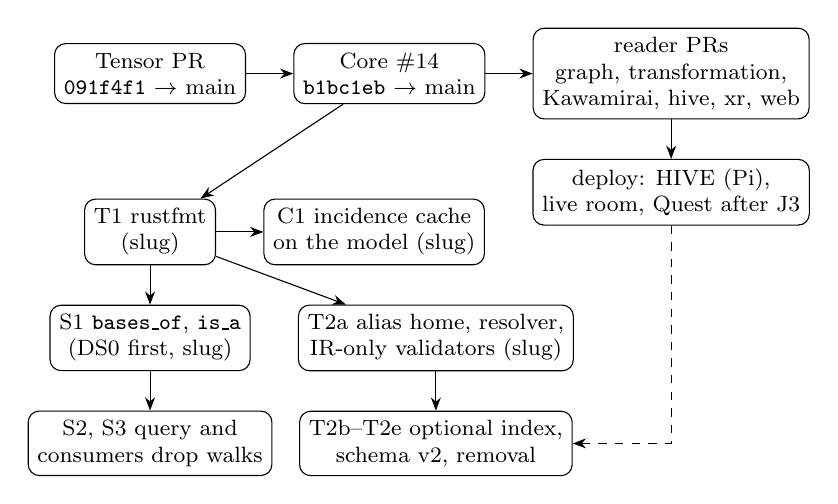
\begin{tikzpicture}[node distance=5mm and 6mm,every node/.style={draw,rounded corners,align=center,font=\footnotesize},>={Stealth}]
\node (tensor) {Tensor PR\\\texttt{091f4f1} $\to$ main};
\node (core) [right=of tensor] {Core \#14\\\texttt{b1bc1eb} $\to$ main};
\node (readers) [right=of core] {reader PRs\\graph, transformation,\\Kawamirai, hive, xr, web};
\node (deploy) [below=of readers] {deploy: HIVE (Pi),\\live room, Quest after J3};
\node (t1) [below=12mm of tensor] {T1 rustfmt\\(slug)};
\node (c1) [right=of t1] {C1 incidence cache\\on the model (slug)};
\node (s1) [below=of t1] {S1 \texttt{bases\_of}, \texttt{is\_a}\\(DS0 first, slug)};
\node (t2a) [right=of s1] {T2a alias home, resolver,\\IR-only validators (slug)};
\node (s2) [below=of s1] {S2, S3 query and\\consumers drop walks};
\node (t2b) [below=of t2a] {T2b--T2e optional index,\\schema v2, removal};
\draw[->] (tensor)--(core); \draw[->] (core)--(readers); \draw[->] (readers)--(deploy);
\draw[->] (core)--(t1); \draw[->] (t1)--(c1); \draw[->] (t1)--(s1); \draw[->] (t1)--(t2a);
\draw[->] (s1)--(s2); \draw[->] (t2a)--(t2b); \draw[->,dashed] (deploy.south) |- (t2b.east);
\end{tikzpicture}

\end{center}

\end{document}
